\documentclass{article}
\usepackage{fancyhdr}
\usepackage{extramarks}
\usepackage{amsmath}
\usepackage{amsthm}
\usepackage{amsfonts}
\usepackage{tikz}
\usepackage[plain]{algorithm}
\usepackage{algpseudocode}

\begin{document}
\author{Chuan Lu}
\title{PHYS:5905 Homework 6}
\maketitle

\medskip

\begin{enumerate}
\item Homework 6a

The result is shown in Figure \ref{hw6a}.

\begin{figure}[h]
\centering
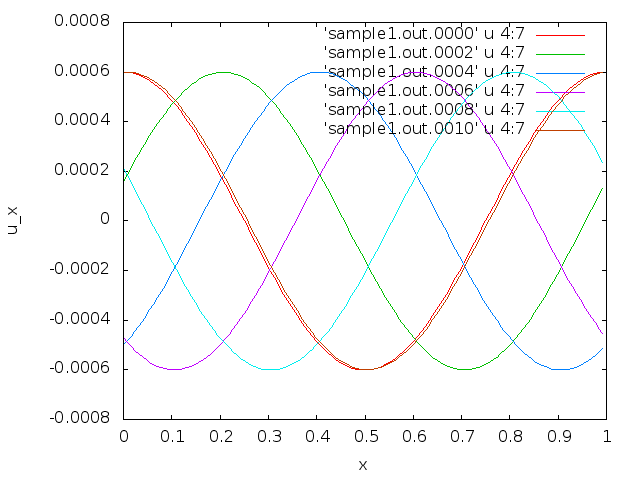
\includegraphics[scale=0.4]{sample.png}
\caption{HW 6(a)}
\label{hw6a}
\end{figure}

\item Homework 6b, 1

The result is shown in Figure \ref{hw6b-1}.

\begin{figure}[h]
\centering
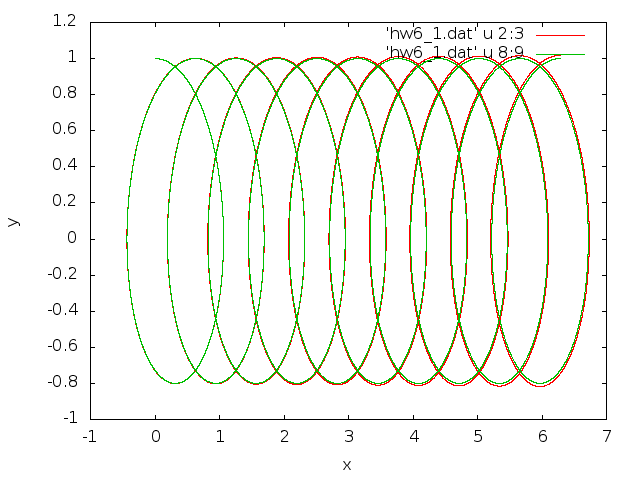
\includegraphics[scale=0.4]{hw6b_1.png}
\caption{HW 6b, 1}
\label{hw6b-1}
\end{figure}

\item Homework 6b, 2

The result is shown in Figure \ref{hw6b-2.1} and \ref{hw6b-2.2}

\begin{figure}[h]
\centering
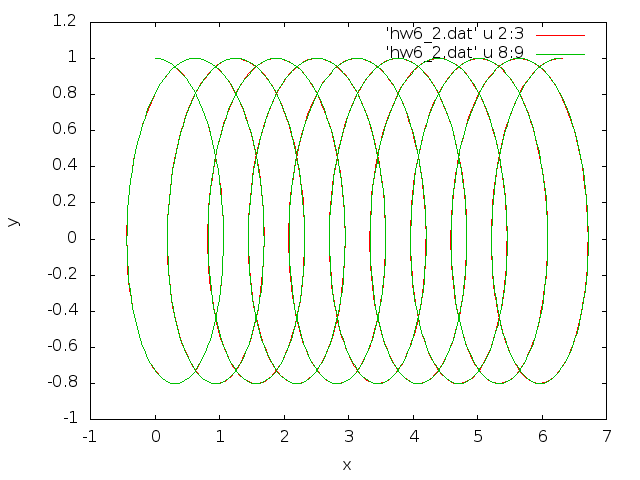
\includegraphics[scale=0.4]{hw6b_2_1.png}
\caption{HW 6b, 2.1}
\label{hw6b-2.1}
\end{figure}

\begin{figure}[h]
\centering
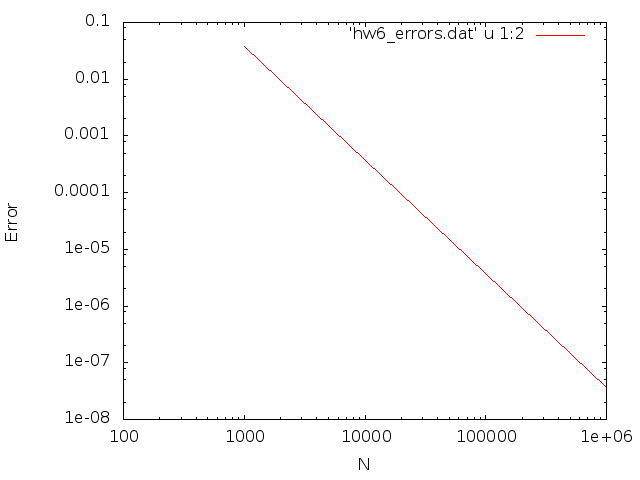
\includegraphics[scale=0.4]{hw6b_2_2.png}
\caption{HW 6b, 2.2}
\label{hw6b-2.2}
\end{figure}

\end{enumerate}

\end{document}